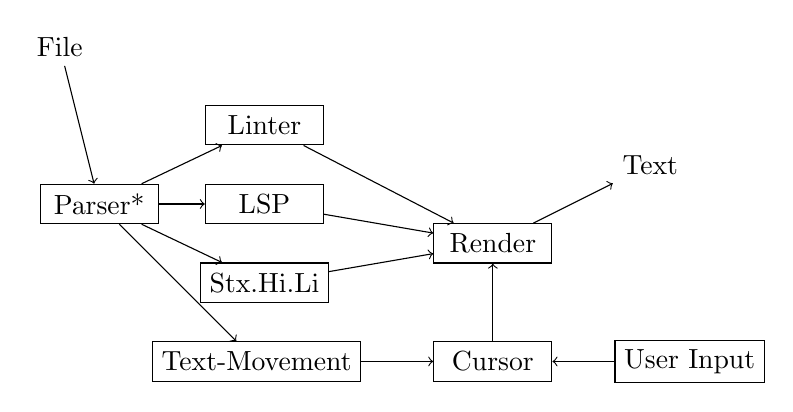
\begin{tikzpicture}
  % Nodes
  \node (file) [] at (-6, 3) {File};
  \node (parser) [rectangle, draw, minimum height=0.5cm, minimum width=1.5cm] at (-5.5, 1) {Parser*};
  \node (lsp) [rectangle, draw, minimum height=0.5cm, minimum width=1.5cm] at (-3.4, 1) {LSP};
  \node (stxhili) [rectangle, draw, minimum height=0.5cm, minimum width=1.5cm] at (-3.4, 0) {Stx.Hi.Li};
  \node (text-movement) [rectangle, draw, minimum height=0.5cm, minimum width=1.5cm] at (-3.5, -1) {Text-Movement};
  \node (linter) [rectangle, draw, minimum height=0.5cm, minimum width=1.5cm] at (-3.4, 2) {Linter};
  \node (cursor) [rectangle, draw, minimum height=0.5cm, minimum width=1.5cm] at (-0.5, -1) {Cursor};
  \node (user-input) [rectangle, draw, minimum height=0.5cm, minimum width=1.5cm] at (2, -1) {User Input};
  \node (render) [rectangle, draw, minimum height=0.5cm, minimum width=1.5cm] at (-0.5, 0.5) {Render};
  \node (text) at (1.5, 1.5) {Text};
  % Arrow
  \draw[->] (file) -- (parser) node[midway, above] {};
  \draw[->] (parser) -- (lsp) node[midway, above] {};
  \draw[->] (parser) -- (stxhili) node[midway, above] {};
  \draw[->] (parser) -- (linter) node[midway, above] {};
  \draw[->] (parser) -- (text-movement) node[midway, above] {};
  \draw[<-] (render) -- (lsp) node[midway, above] {};
  \draw[<-] (render) -- (stxhili) node[midway, above] {};
  \draw[<-] (render) -- (linter) node[midway, above] {};
  \draw[<-] (cursor) -- (text-movement) node[midway, above] {};
  \draw[<-] (cursor) -- (user-input) node[midway, above] {};
  \draw[->] (cursor) -- (render) node[midway, above] {};
  \draw[->] (render) -- (text) node[midway, above] {};
\end{tikzpicture}

